\documentclass[12pt,a4paper,notitlepage]{article}

\usepackage[utf8]{inputenc}

\usepackage[francais]{babel}\usepackage[T1]{fontenc}
\usepackage[cyr]{aeguill}
\usepackage{lmodern}
\usepackage{color}
\usepackage{boites}
\usepackage{caption}
\usepackage{fancybox}
\usepackage{listings}
\usepackage{multicol}
\usepackage[table]{xcolor}

\usepackage[T1]{fontenc}
\usepackage[scaled]{helvet}
\renewcommand*\familydefault{\sfdefault}

%\lstset{language=bash, basicstyle=\footnotesize, frame=shadowbox, rulesepcolor=\color{gris}, captionpos=b}

  \lstset{
         basicstyle=\footnotesize\ttfamily, % Standardschrift
         %numbers=left,               % Ort der Zeilennummern
         numberstyle=\tiny,          % Stil der Zeilennummern
         %stepnumber=2,               % Abstand zwischen den Zeilennummern
         numbersep=5pt,              % Abstand der Nummern zum Text
         tabsize=2,                  % Groesse von Tabs
         extendedchars=true,         %
         breaklines=true,            % Zeilen werden Umgebrochen
         keywordstyle=\color{red},
                frame=b,         
         keywordstyle=[1]{\itshape}{//},    % Stil der Keywords
         stringstyle=\color{white}\ttfamily, % Farbe der String
         showspaces=false,           % Leerzeichen anzeigen ?
         showtabs=false,             % Tabs anzeigen ?
         xleftmargin=5pt,
         framexleftmargin=1pt,
         framexrightmargin=5pt,
         %numbers=left,
         frame=toplines,
         framextopmargin=3pt,
       %  framexleftmargin=8pt,
         numberblanklines=false,
         %morecomment=[s][marron]{/*}{*/},
         %moredelim=*[s][\color{blue}]{/*}{*/}
         %morecomment=[s][marron]{/*-}{*/}},         
         framexbottommargin=5pt,
         captionpos=b,
         %backgroundcolor=\color{lightgray},
         showstringspaces=false      % Leerzeichen in Strings anzeigen ? 
 }

\DeclareCaptionFont{white}{\color{white}}
\DeclareCaptionFormat{listing}{\colorbox[cmyk]{0.43, 0.35, 0.35,0.01}{\parbox{\textwidth}{\hspace{10pt}#1#2#3}}}
\captionsetup[lstlisting]{format=listing,labelfont=white,textfont=white, singlelinecheck=false, margin=0pt, font={bf,footnotesize}}

\definecolor{gris}{gray}{0.75}
\definecolor{bleup}{HTML}{258EE9}


%\renewcommand*\familydefault{\ttdefault} %% Only if the base font of the document is to be typewriter style
%\renewcommand{\rmdefault}{ptm}


\usepackage[
   pdfauthor={Ludovic Terrier & Arnaud Goulut},
   pdftitle={RE12 - TP6},
   ]{hyperref}
   
   
\usepackage[pdftex]{graphicx}

%\usepackage{titlesec}
%\titleformat{\section}[frame] {\normalfont} {\filright
%\footnotesize
%\enspace\textbf{\thesection}\enspace} {8pt} {\Large\bfseries\filcenter}

%% Je contrôle la taille de ma zone imprimée...
\usepackage{anysize}
%% ...en définissants les marges {gauche}{droite}{haute}{basse}
\marginsize{25mm}{15mm}{10mm}{15mm}

\begin{document}

\title{Gestion de réseau par SNMP}
\author{Arnaud Goulut et Ludovic Terrier}
\date{Juin 2010}
\maketitle


%\tableofcontents

\thispagestyle{empty}


 
%%%%%%%%%%%%%%%%%%%%%%%%%%%%%%%%%%% 1ère partie
\section{Configuration et prise en main de l'agent SNMP}
\subsection{Installation d'un agent}
L'agent net-snmp est déjà installé sur les machines. Cependant il reste à installer les utilitaires en ligne de commande afin d'effectuer les tests qui suivront, via la commande :\\


\noindent \texttt{yum install net-snmp-libs net-snmp-utils}

\paragraph{}Le paquet net-snmp-utils regroupe l'ensemble des outils nécessaire pour tester le bon fonctionnement de la supervision de son réseau tel que : snmpwalk, snmpget\ldots 

\subsection{Ligne de commande}
Nous allons dans cette partie, décrire le fonctionnement ainsi qu'un exemple d'utilisation des outils cités ci-dessus.

\subsubsection{snmpwalk}
Cet outil permet de récupérer des informations à partir d'un point donné dans l'arbre de représentation des OIDs. Pour cela il utilise les requêtes \texttt{get-next-request} et \texttt{get-response} afin de récupérer en suivant tous les items (pas très jolie cette phrase).

\subsubsection{snmpget}
Snmpget permet quant à lui de récupérer uniquement la valeur d'un OID précisé, sans déroulé l'arbre. Ainsi, si nous voulons récupérer la personne à contacter pour un équipement précisé on utilisera :\\

\noindent \texttt{snmpget -v 2c -c publicB3 127.0.0.1 1.3.6.1.2.1.1.4.0}

\subsubsection{snmpgetnext}
Cet outil permet de récupérer la valeur de l'OID suivant celui que l'on va donner en paramètre. Ainsi pour récupérer la valeur de l'uptime en donnant l'OID situé avant dans l'arbre :\\

\noindent \texttt{snmpgetnext -v 2c -c publicB3 127.0.0.1 1.3.6.1.2.1.1.2}

\subsubsection{snmptable}
Cet outil permet de récupérer un ensemble d'informations en une seule commande, en le mettant sous forme d'un tableau :\\

\begin{lstlisting}[title=Résultat snmptable pour les connexions TCP]
root@pc05-d202 snmp]# snmptable -v 1 -c publicB3 127.0.0.1 1.3.6.1.2.1.6.13
SNMP table: TCP-MIB::tcpConnTable

tcpConnState tcpConnLocalAddress tcpConnLocalPort tcpConnRemAddress tcpConn
    listen             0.0.0.0              111           0.0.0.0        0
    listen             0.0.0.0            10000           0.0.0.0        0
    listen             0.0.0.0            48781           0.0.0.0        0
    listen           127.0.0.1               25           0.0.0.0        0
    listen           127.0.0.1              199           0.0.0.0        0
  established      192.168.3.1            39628     188.165.75.23       22
\end{lstlisting}

\subsection{MibBrowser}
Ce logiciel permet de visualiser graphiquement l'ensemble de l'arbre et des valeurs associées à chaque OID.

\paragraph{} Le logiciel ne fonctionnait pas très bien, en effet en utilisant la fonction snmpget, il parcourait l'ensemble de l'arborescence au lieu de s'arrêter.

\section{Surveillance des équipements réseau et alarmes}
\subsection{Configuration équipements}
Nous avons donc tu configurer les agents SNMP de nos équipements afin d'utiliser SNMP.\\
\begin{lstlisting}[title=Commandes Cisco pour configurer l'agent SNMP du routeur]
Router3(config)# snmp-server contact Arnaud Goulut
Router3(config)# snmp-server location Salle de TP, D202
Router3(config)# snmp-server community publicB3
\end{lstlisting}

\paragraph{} Pour vérifier le bon fonctionnement, on utilise snmpwalk pour récupérer les informations de la partie \texttt{system} de la MIB :

\begin{lstlisting}[title=Vérification du fonctionnement SNMP sur le routeur]
root@pc05-d202# snmpwalk -v 2c -c publicB3 192.168.3.126 1.3.6.1.2.1.1
SNMPv2-MIB::sysDescr.0 = STRING: Cisco IOS Software, 2800 Software
Technical Support: http://www.cisco.com/techsupport
SNMPv2-MIB::sysObjectID.0 = OID: SNMPv2-SMI::enterprises.9.1.576
DISMAN-EVENT-MIB::sysUpTimeInstance = Timeticks: (682232) 1:53:42.32
SNMPv2-MIB::sysContact.0 = STRING: Arnaud
SNMPv2-MIB::sysName.0 = STRING: Routeur3
SNMPv2-MIB::sysLocation.0 = STRING: salle de tp
\end{lstlisting}

\subsection{Perte de connectivité}
Sur nos équipement, on doit donc activer l'émission de trap pour prévenir directement notre serveur de supervision.

\begin{lstlisting}[title=Activation des traps pour l'état des liens]
Router3(config)# snmp-server host 192.168.3.1 version 2c publicB3
Router3(config)# snmp-server enable traps snmp linkdown linkup coldstart warmstart
\end{lstlisting}

\subsection{Le démon snmptrapd}
dfdfklsjfkj

\section{Prise en main d'une console de supervision}
\subsection{Installation de ZenOSS}
Ce fichier définit l'ensemble des options du protocole SIP qui seront utilisées lorsque notre serveur de téléphonie sera en fonctionnement. \\
\begin{lstlisting}[title=sip.conf v1]
[user1]
username=user1
\end{lstlisting}

\subsection{Parcours des fonctionnalités}

Dans \textit{Asterisk}, les extensions définissent une série d'étapes uniques qui vont être déroulées au cours d'un appel. Pour définir une extension, on utilise la forme : \\

%\paragraph{}Voici le schéma décrivant l'infrastructure du réseau que nous désirons obtenir :
%\clearpage%
%\begin{figure}[!h]
%\begin{center}
%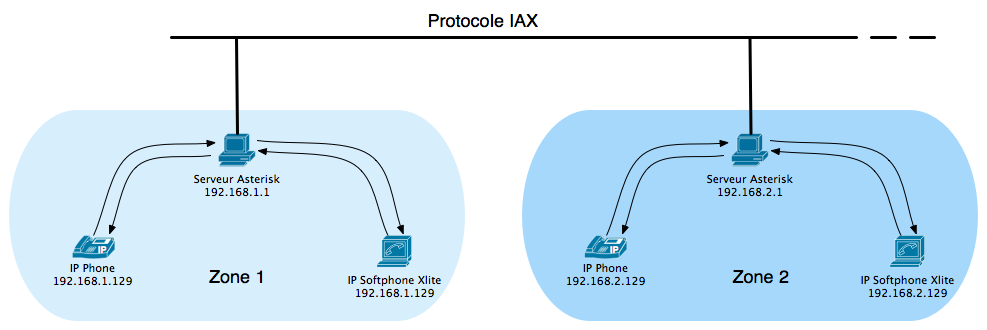
\includegraphics[height=5cm]{structure_reseau_IAX}
%\caption{Structure du réseau}
%\label{fig:da}
%\end{center}
%\end{figure}
\end{document}